% figures-es/funnel-awareness-to-purchase.tex
% Standalone TikZ: funnel de marketing (Conciencia -> Consideración -> Compra).
% Compilado a figures-es/funnel-awareness-to-purchase.pdf via tools/build-figures-es.sh.
\documentclass[tikz,border=4pt]{standalone}
\usepackage{tikz}
\usetikzlibrary{arrows.meta,positioning}

% Paleta coincidente con los colores de tcolorbox de preamble.sty
\definecolor{topblue}{HTML}{1A5276}
\definecolor{midteal}{HTML}{0E6655}
\definecolor{botgreen}{HTML}{117A65}

\begin{document}
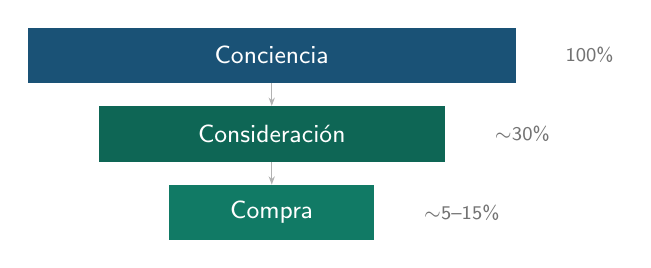
\begin{tikzpicture}[
    bar/.style={draw=none, fill=#1, text=white, font=\small\sffamily,
                minimum height=7mm, inner sep=2pt, align=center},
    note/.style={font=\scriptsize\sffamily, text=black!55},
]
  \node[bar=topblue, minimum width=62mm] (aw) at (0,0)     {Conciencia};
  \node[bar=midteal, minimum width=44mm] (co) at (0,-10mm) {Consideración};
  \node[bar=botgreen, minimum width=26mm] (pu) at (0,-20mm) {Compra};

  \node[note, right=5mm of aw] {100\%};
  \node[note, right=5mm of co] {$\sim$30\%};
  \node[note, right=5mm of pu] {$\sim$5--15\%};

  \draw[-{Stealth[length=3pt]}, gray!60] (aw.south) -- (co.north);
  \draw[-{Stealth[length=3pt]}, gray!60] (co.south) -- (pu.north);
\end{tikzpicture}
\end{document}
